\documentclass{article}
\usepackage[utf8x]{inputenx}
\usepackage{graphicx}
\newcommand{\uncl}[1]{${\wr}$#1${\wr}$}

\begin{document}
\parindent0em

\begin{center}\textbf{Notes on Śivadharma/Vṛṣasārasaṃgraha MSS}:

\end{center}

Does the Wellcome MS (WI $\delta$16 I–VIII; here: L) copy NGMPP A 1082/3\\
 (here: N) directly?

\bigskip

N reads 

[\textit{spha}]\textit{ṭikāṃ×ram} [= \textit{°kāṃbaram}] \textit{eva ca} $|$
\textit{daśayogāsanāsīno}:
\smallskip

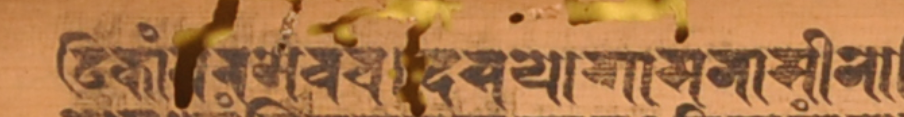
\includegraphics[scale=.4]{dasayoga_msNa.png}
\medskip

L gives

\textit{sphaṭikāṃsatam eva ca $||$ devayogāsanāsīto}

supplying \textit{sa} for the lost syllable and misreading the 
damaged \textit{da} as \textit{de} and the \textit{śa} as \textit{va}:
\smallskip

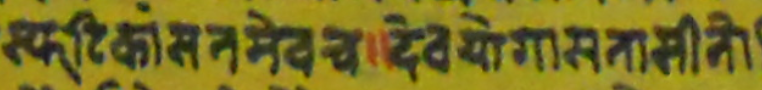
\includegraphics[scale=.4]{dasayoga_msL.png}

\bigskip
\hrule
\bigskip

Here N reads

[\textit{japo yogas tapo}] \textit{dhyānaṃ svādhyāyaś ca} 

with \textit{dhyā} and \textit{svā} damaged:

\smallskip
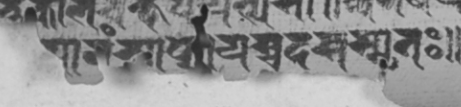
\includegraphics[scale=.7]{japoyoga_msNa.png}
\medskip

L cannot read the bit that is completely lost, and it misreads 
the damaged \textit{dhyānaṃ} as \textit{dhānaṃ}, \textit{svādhyā} as \textit{sādhu}:
\smallskip

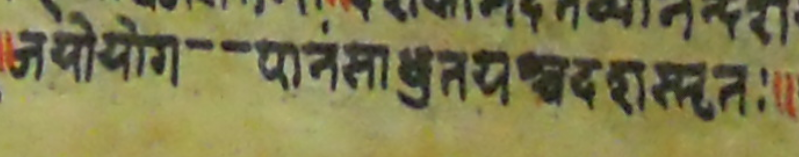
\includegraphics[scale=.4]{japoyoga_msL.png}

\vfill\pagebreak

Here the text is supposed to read\\ 
\textit{kare gṛhya tapodhanam $|$ tataḥ so 'ntarhitas{ }tatra tenaiva}.

N gives\\
\textit{x x x x x x dha\uncl{na tataḥ so 'ntar}hitas tatra tenaiva}
\medskip

\leftskip-8em
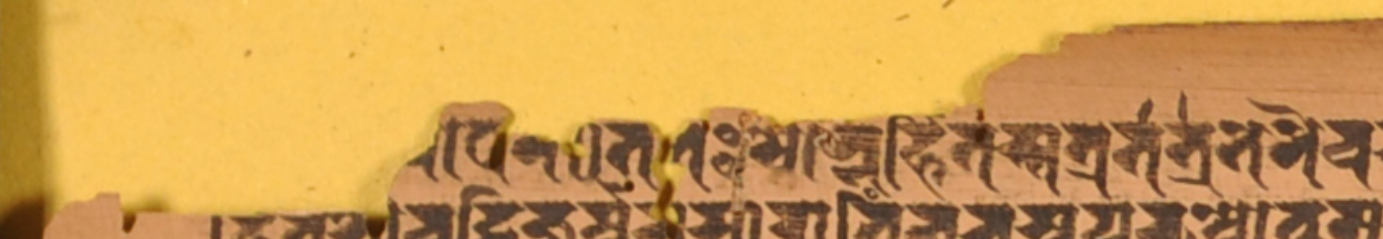
\includegraphics[scale=.4]{/home/csaba/indology/dharma_project/beamer_prezi/pondy/hitas_msNa.png}

\medskip

\leftskip0em
L gives\
\textit{kare - - - dhatāṃ tataḥ $||$ sati hitas tatra tenaiva}

\medskip
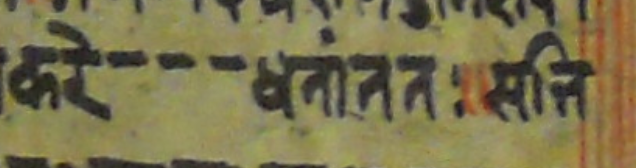
\includegraphics[scale=.4]{/home/csaba/indology/dharma_project/beamer_prezi/pondy/hitas01_msL.png}
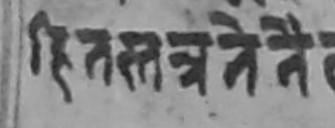
\includegraphics[scale=.4]{/home/csaba/indology/dharma_project/beamer_prezi/pondy/hitas02_msL.png}





\end{document}
